\documentclass{article}
\usepackage[education, final]{neurips_2026}

\usepackage[utf8]{inputenc}
\usepackage[T1]{fontenc}
\usepackage{hyperref}
\usepackage{url}
\usepackage{amsfonts}
\usepackage{microtype}
\usepackage{graphicx}

\setcitestyle{numbers,square,comma}

\title{Generate, then verify: pairing a molecular generative\\model with the checks that can fail it}

\author{%
  Noah Flynn\\
  University of California, Berkeley\\
  \texttt{noahrflynn.com}\\
  \url{https://github.com/nrflynn2/generate-then-verify}
}

\begin{document}

\maketitle

\section{The concept}

A model that invents molecules is half a system. The other half decides whether the thing could
exist: whether its atoms sit at distances physics allows, whether a second, independent method puts
it in the same place on the target protein, whether a scoring model will say it sticks at all. Teach
only the first half and a learner produces candidates and cannot tell a real one from a rendering.
This resource teaches the pair as one loop.

Diffusion arrived in 2020 and flow matching in 2022; both are settled machinery, and neither is the
lesson. Filtering generated molecules is older still: drug-likeness rules, docking and
synthetic-accessibility scores have screened candidates for decades. What is new between 2023 and
2026 is narrower, and it is the lesson: a named, reproducible verification stack reported beside the
generator as one system. The strain-and-interaction instrument arrived in
2023~\citep{harris2023posecheck}, the geometry battery in 2024~\citep{buttenschoen2024posebusters},
and by 2025 a co-folding model that is itself a verifier with its own failure
modes~\citep{passaro2025boltz2}. By 2026 a generator is introduced by the battery it
passes~\citep{vonessen2025tabasco,cremer2026flowr}. The samplers are scaffolding a learner passes
through on the way there.

Taught as a loop, the failures become the curriculum. Twenty designs generated inside a protein
pocket are all valid graphs and fifteen pass the full physical battery, but the receptor file holds
2,250 protein atom records and no cofactor or water records, so six of the nine intermolecular checks
could not have failed. Learners discover that by measuring the file.

\section{Leveling and prerequisite knowledge}

Advanced undergraduate for modules 1 to 3, graduate for modules 4 to 8. Required: Python fluency at
the level of reading a function and indexing a DataFrame, and basic probability. Helpful but not
required: that a network is trained by minimizing a loss, and what an ordinary differential equation
is. No chemistry or structural biology is assumed: the vocabulary is short, each term is defined at
first use and in the glossary, and every model a module uses is introduced, with lecture time
budgeted, before it runs. No GPU, no key, no network.

\section{Learning objectives and outcomes}

Twenty-four objectives map one to one onto the eight modules and the twelve assessed exercises, X1 to
X12, each naming an action a learner can be observed doing. Two of the twenty-four: \textbf{Audit} a
published verification table by measuring the receptor file instead of trusting the table, and find
the checks that could not have failed (M4, X5). \textbf{Compute} a potency estimate outside its
calibrated range and observe a rejected molecule outrank a known drug (M7, X10).

\begin{figure}[t]
\centering
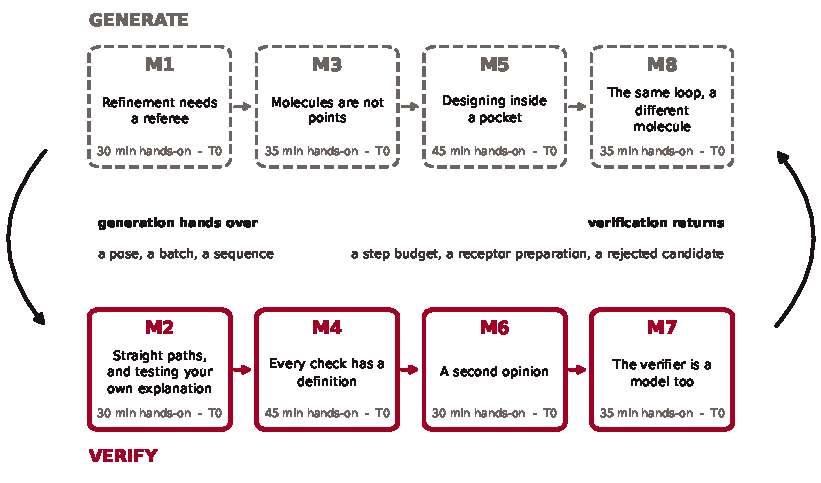
\includegraphics[width=66mm]{module_map_panelA.pdf}
\caption{The eight modules on the generate-then-verify spine. Every module carries both halves of the
loop, so verification starts in the first fifteen minutes rather than in module five, and every cached
path runs on a laptop CPU, no accelerator required.}
\end{figure}

\section{What the checks can and cannot show}

Six third-party tools make up the stack~\citep{harris2023posecheck,buttenschoen2024posebusters,schneuing2024diffsbdd,passaro2025boltz2,vonessen2025tabasco,cremer2026flowr};
each is read here for what it verifies, and each has a limit a learner meets directly. The battery is
physical and geometric. It is not a binding assay. PoseBusters passes a pose with valid bonds, sensible
rings and no steric clashes; it does not say the molecule binds, and a graph-validity score says even
less. A check fires only against atoms that are present: against the cofactor-free receptor above, six
of the nine intermolecular checks are vacuous and pass by default. Model verifiers add their own
limits; the Boltz-2 affinity head, calibrated on measured complexes, scores a rejected design above a
known drug when read on de novo molecules (X10). A second method is independent evidence only when it
can fail differently: the re-docking in module 6 and the DiffSBDD generator it checks are both
equivariant diffusion models trained on PDB-derived complexes, so agreement between them would be
correlated by construction rather than independent. Here they disagree anyway: median 4.4\,\AA{},
none within 2\,\AA. Learners are taught to ask what a verifier shares with the generator before
counting its agreement.

\section{Teaching materials, originality and attribution}

The curriculum layer is new and published nowhere else: an eight-module lesson guide, instructor
notes, the objectives and prerequisite map, an assessment blueprint, a 54-term glossary, a literature
bridge and Figure 1. The exercise set is also new: twelve assessed tasks plus an environment check,
across four notebooks with worked solutions in a separate directory, 151 minutes of learner work,
running in about 73 seconds on a CPU. The substrate the notebooks read is earlier work:
seventeen cached result files drawn from a larger set produced for the author's prior published
material, so a learner reproduces every number on a laptop. Every file carries one of three provenance
values in \texttt{MANIFEST.json}, so the boundary between new and reused is checkable. Three
configurations are pre-cut: a 60-minute seminar, a 90-minute lab and a four-week module. CC BY 4.0,
code Apache 2.0. The package is validated for reproducibility but has not been run in a classroom; learning-outcome
data is the first open problem. The second is a verifier that shares none of the generator's training
priors. A learner who finishes can read
the results table of a NeurIPS talk on molecular or protein generation and ask the three questions
that decide it: which physical checks ran and against which receptor preparation, whether a second
method agreed and by how much, and whether the affinity or similarity number is inside the range where
it means something.


\footnotesize
\begin{thebibliography}{9}
\setlength{\itemsep}{0pt}\setlength{\parskip}{0pt}
\bibitem{harris2023posecheck} C. Harris et al. Benchmarking generated poses in structure-based drug design. arXiv:2308.07413, 2023.
\bibitem{buttenschoen2024posebusters} M. Buttenschoen et al. PoseBusters: AI-based docking methods fail to generate physically valid poses. \emph{Chem. Sci.} 15:3130-3139, 2024.
\bibitem{schneuing2024diffsbdd} A. Schneuing et al. Structure-based drug design with equivariant diffusion models. \emph{Nat. Comput. Sci.}, 2024. doi:10.1038/s43588-024-00737-x
\bibitem{passaro2025boltz2} S. Passaro et al. Boltz-2: towards accurate and efficient binding affinity prediction. \emph{bioRxiv} 2025.06.14.659707, 2025.
\bibitem{vonessen2025tabasco} C. Vonessen et al. TABASCO: a fast, simplified model for molecular generation. arXiv:2507.00899, 2025.
\bibitem{cremer2026flowr} J. Cremer et al. FLOWR: flow matching for structure-aware ligand generation. \emph{Nat. Comput. Sci.}, 2026. doi:10.1038/s43588-026-00998-8
\end{thebibliography}

\end{document}
